\chapter{Means Comparison}\label{ch:mc}
\section{Methods}
\subsection{Introduction}
\begin{itemize}
    \item In the year 2008 scrubbers were installed into the Bullrun and kingston power plants
    \item These scrubbers significantly reduced the amount of SO$_4$ emitted by the smoke stacks of the power plants by {\bf how much}
    \item A the same time an obvious decrease in measured SO$_4$ was discovered in the Stream Survey samples \citep{annualreport2012}.
   \begin{figure}[h!]
  \centering
  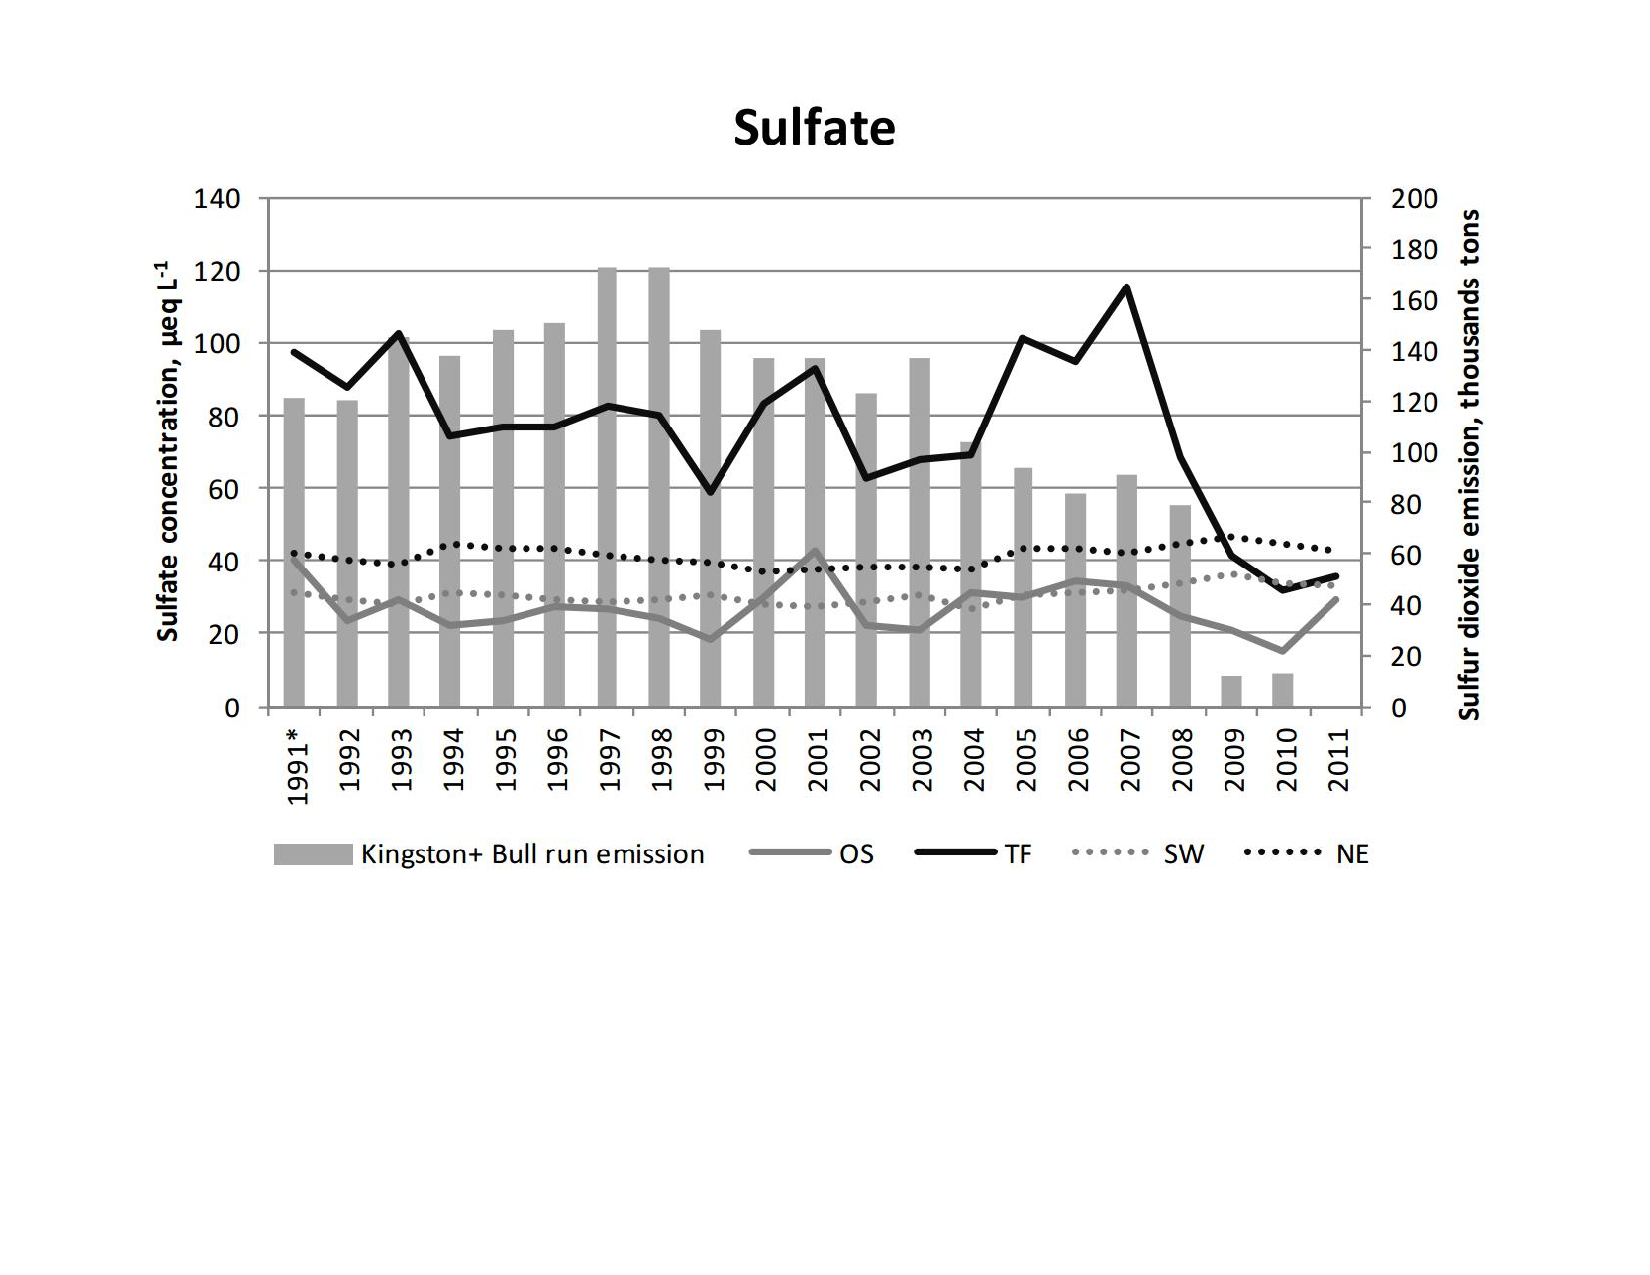
\includegraphics[width=6in]{SulfateEmissions}\\
  \caption{Sulfate emmisions of Kingstion and Bull run against those measured in Noland high elevation site.}\label{fig:sulfateemissions}
\end{figure}
    \item The amount of SO$_4$ in the streams is thought to be (correlated with?) to the pH index of the streams when the SO$_4$ goes up the pH goes down.
    \item The hypothesis is that of the three sets of data containing water quality measurements from 1993 to 2012, if the data is broken at 2002 and 2008, that
    because of the obvious measured decrease in SO$_4$, there will be an obvious difference of means in the sets before and after 2008.
    \item This can be tested using an Analysis of Variance procedure.
    \item The data is only pH measurements for the three sets
    \subsubsection{Instruments}
    \begin{itemize}
        \item The program used for this procedure was (probably SAS).
        \item Heterscedasticity can be a problem a brown-forsythe test was employed to test for this.
        \item If three groups are analyzed using ANOVA the only two outcomes may be "they are different" or "they are not different".
        \item If they are not different then the analysis of the data is over.
        \item If they are different then it would be nice to know which sets are different.
        \item This is accomplished with a Bonferoni analysis
    \end{itemize}
\end{itemize}
\subsection{Bonferoni Introduction}
\begin{itemize}
    \item Introduction from text book.
    \item rank-sum
    \subsubsection{instruments}
    \begin{itemize}
        \item Bonferoni can output a graph presenting the means of each group in order to visually check for a difference in means. It will also output 95\%
        confidence intervals between each pair of groups.  This way definitive answers can be found for the question of "are they or are they not the same?"
        \item Bonferoni assumptions
        \item SAS
    \end{itemize}
\end{itemize}
\section{Results}
\begin{itemize}
	\item Background info?
	\item The output of the Bonferoni method includes 95\% confidence intervals that represent definitive comparisons of the means of two groups of data.  If the C.I. includes zero then the means are not statistically different.
	\begin{table}[htbp]
\caption{Bonferroni comparisons between multiple groups}
\begin{center}
\begin{tabular}{p{2cm}cccccccccccc}
\toprule
 Elevation Classes& \multicolumn{ 3}{c}{pH} & \multicolumn{ 3}{c}{ANC} & \multicolumn{ 3}{c}{Nitrate} & \multicolumn{ 3}{c}{Sulfate} \\ \cline{2-13}\noalign{\smallskip}
 & \multicolumn{ 1}{c}{1-2} & 1-3 & 2-3 & 1-2 & 1-3 & 2-3 & 1-2 & 1-3 & 2-3 & 1-2 & 1-3 & 2-3 \\  \cline{2-13}
\multicolumn{1}{c}{1} & \textbf{$\neq$} & \textbf{$\neq$} & \textbf{$\neq$} & \textbf{=} & \textbf{=} & \textbf{=} & \textbf{$\neq$} & \textbf{=} & \textbf{=} & \textbf{=} & \textbf{=} & \textbf{=} \\ 
\multicolumn{1}{c}{2} & \textbf{=} & \textbf{=} & \textbf{=} & \textbf{=} & \textbf{$\neq$} & \textbf{=} & \textbf{$\neq$} & \textbf{$\neq$} & \textbf{=} & \textbf{$\neq$} & \textbf{$\neq$} & \textbf{=} \\ 
\multicolumn{1}{c}{3} & \textbf{$\neq$} & \textbf{$\neq$} & \textbf{$\neq$} & \textbf{=} & \textbf{$\neq$} & \textbf{=} & \textbf{=} & \textbf{$\neq$} & \textbf{$\neq$} & \textbf{=} & \textbf{=} & \textbf{=} \\ 
\multicolumn{1}{c}{4} & \textbf{=} & \textbf{$\neq$} & \textbf{$\neq$} & \textbf{=} & \textbf{=} & \textbf{=} & \textbf{=} & \textbf{=} & \textbf{=} & \textbf{=} & \textbf{=} & \textbf{=} \\ 
\multicolumn{1}{c}{5} & \textbf{$\neq$} & \textbf{$\neq$} & \textbf{$\neq$} & \textbf{=} & \textbf{$\neq$} & \textbf{$\neq$} & \textbf{$\neq$} & \textbf{=} & \textbf{$\neq$} & \textbf{=} & \textbf{=} & \textbf{=} \\ 
\multicolumn{1}{c}{6} & \textbf{=} & \textbf{$\neq$} & \textbf{$\neq$} & \textbf{=} & \textbf{=} & \textbf{=} & \textbf{=} & \textbf{=} & \textbf{=} & \textbf{=} & \textbf{=} & \textbf{=} \\ 
\bottomrule
\end{tabular}
\end{center}
\label{tab:Bontable}
\end{table}%needs cleaning
	\item \autoref{tab:Bontable} reports the Bonferoni comparison means between the four water quality variables(pH, ANC, NO$_3$, SO$_4$) in one time set against the same water quality variable in another time set by elevation bands.
	\item There are three groups compared in \autoref{tab:Bontable}, they are the three time sets: 93-02, 03-08, 09-12.  The table uses = and $\neq$ to represent equality or inequality between the means of the groups compared.
	\item stuff from first draft
	\item the bonferoni analysis also outputs the results in figure form.  These figures visually represent the group means and are presented in \autoref{fig:ANOVApH1} through \autoref{fig:ANOVASO46}.%links in pdf work but produce figure ??
	\item The negative trend of ANC is something to take note of.
\end{itemize}
\section{Discussion}
\begin{itemize}
	\item Are these results a special case?
	\item Do these differences show up in other water quality analyses, not in the S.S.?
	\item What are the reasons that the means are higher or lower than expected?
	\item Differences between sets 2 and 3 were expected due to the scrubbers, did this occur?
	\item Why aren't the results as clear as the chart in the \citep{cai2012}?
	\begin{itemize}
		\item probably math
	\end{itemize}
	\item General hypothosis about what the results suggest
	\begin{itemize}
		\item The results suggest that a larger difference is needed to see a sulfate difference between sets 2 and 3.
	\end{itemize}
\end{itemize}